\documentclass{article}
\usepackage[utf8]{inputenc}
\usepackage{subcaption}
\usepackage{graphicx}
\usepackage[margin=2.5cm]{geometry}
\usepackage{array}
\usepackage{wrapfig}
\usepackage{multirow}
\usepackage{tabularx}
\usepackage{amsmath}
\usepackage{wrapfig}
\usepackage{mathtools}
\usepackage[table]{xcolor}
\usepackage{xcolor,colortbl}
\usepackage{multirow}
\usepackage{polski}
\title{Sprawozdanie 2}

\author{Jan Bronicki \\
Nr indeksu: 249011\\
Marcin Radke\\
Nr indeksu: 241554\\
Ćwiczenie: 8}
\date{}
\begin{document}

\maketitle
%------------------------------------------------------------------
% WSTEP TEORETYCZNY
\section{Wstęp Teoretyczny}
\par Pomiar współczynnika lepkości $\eta$ cieczy metodą Stokesaza za pomocą 
szerokiego cylindrycznego 
naczynia szklanego. \\
\begin{center}
    $
    \eta=\frac{d^{2}\cdot g\cdot t\cdot (\rho_{k}-\rho_{c})}{18h}
    $
    \begin{flushleft}
        Gdzie:\\
        $d$ - średnica kulki\\
        $g$ - przyspieszenie ziemskie $(9.81\frac{m}{s^{2}})$\\
        $\rho_{k}$ - gęstość kulki\\
        $\rho_{c}$ - gęstość cieszy (gliceryny)\\
        $h$ - długość trasy tonącej w glicerynie kulki
    \end{flushleft}
\end{center}
\par Lepkość zostanie wyznaczona na podstawie danych otrzymanych przez obserwacje kulki 
tonącej w glicerynie. Dzięki analizie ruchu kulki, znając jej parametry takie 
jak masa i średnica, które przekładają się na gęstość. Można zanalizować siły oporu,
które stawia ciecz co przekłada się na współczynnik lepkości $\eta$.\\ \\
W naszym eksperymencie wykorzystamy następujące przyrządy:\\
\begin{itemize}
    \item Naczynie cylindryczne z badaną cieczą (w tym wypadku z gliceryną)
    \item Areometr do zbadania gęstości cieczy
    \item Trzy różne kolorowe kulki (Biała, Czarna i Niebieska)
    \item Waga
    \item Suwmiarka do pomiaru średnicy kulek
    \item Stoper
    \item Linijka z podziałką milimetrową
\end{itemize}
% WSTEP TEORETYCZNY
%------------------------------------------------------------------
\newpage
%------------------------------------------------------------------
% OTRZYMANE POMIARY I ICH OPRACOWANIE
\section{Otrzymane pomiary i ich opracowanie}

\begin{figure}[h]
 
    \begin{subfigure}{0.5\textwidth}
        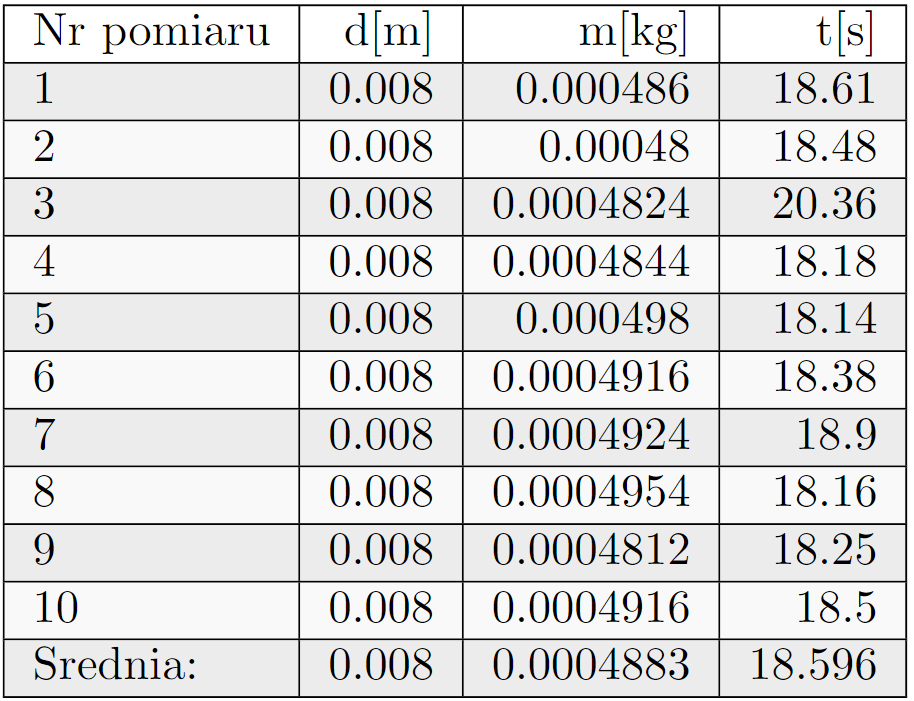
\includegraphics[width=0.9\linewidth, height=5cm]{t_biala_pom.png} 
        \caption{Pomiary kulki Białej}
        \label{fig:subim1}
    \end{subfigure}
    \begin{subfigure}{0.5\textwidth}
        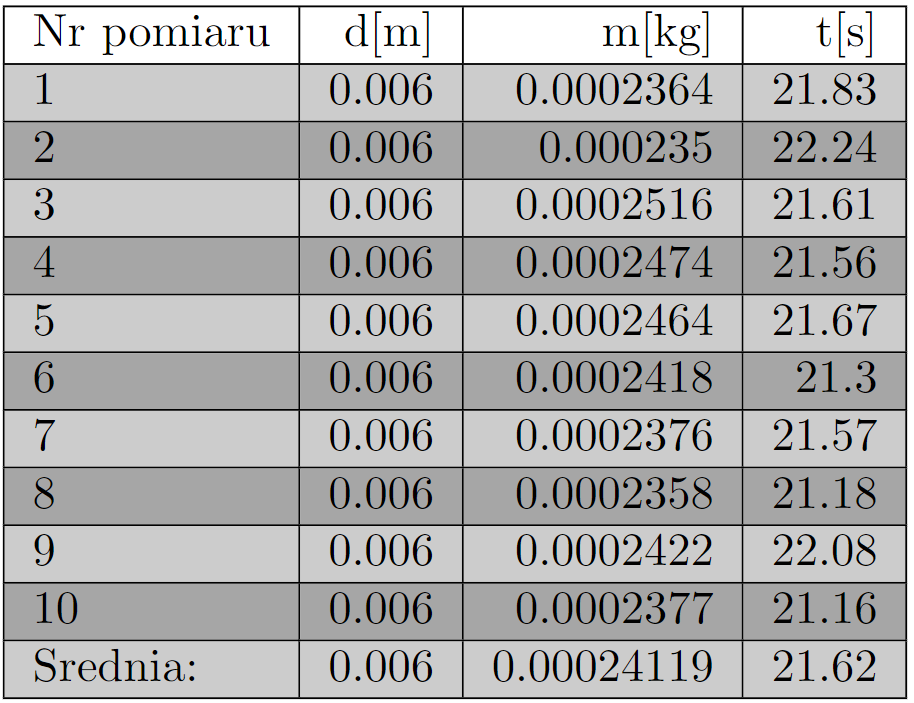
\includegraphics[width=0.9\linewidth, height=5cm]{t_czarna_pom.png}
        \caption{Pomiary kulki Czarnej}
        \label{fig:subim2}
    \end{subfigure}
    \begin{center}
        
        \begin{subfigure}{0.5\textwidth}
            \centering
        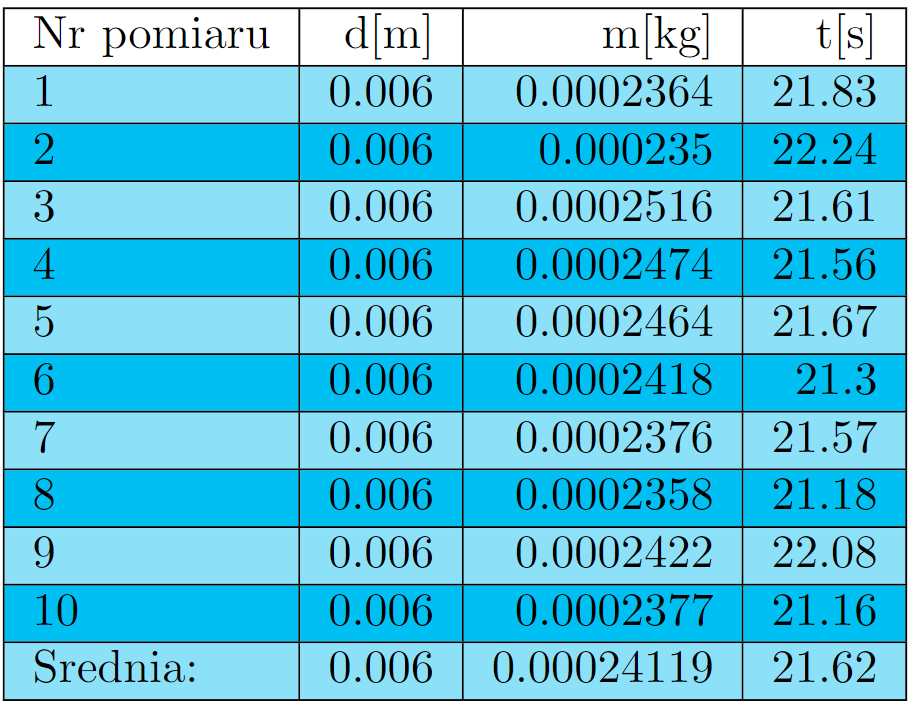
\includegraphics[width=0.9\linewidth, height=5cm]{t_niebieska_pom.png}
        \caption{Pomiary kulki Niebieskiej}
        \label{fig:subim2}
    \end{subfigure}
    \end{center}     
    % \caption{Caption for this figure with two images}
    % \label{fig:image2}
\end{figure}

Gęstość cieczcy została wyznaczona Areometrem:\\
$\rho_{c}=1330 \pm10 \ \left[\frac{kg}{m^{3}}\right]$\\
Gęstość kulki obliczamy z następującego wzoru:\\
$\rho_{k}=\frac{6m}{\pi d^{3}}$\\
Niepewność gęstości kulki:\\
$u_{c}(\rho_{k})=\sqrt{\left(\frac{6}{\pi d^{3}}\right)^{2}\cdot u^{2}(\bar{m}) + \left(\frac{12m}{\pi d^{4}}\right)\cdot u^{2}(d)}$\\
Wzór na niepewność lepkości:\\
$u(\eta)_{c}=u_{c}(y)=\sqrt{\sum^{k}_{j=1}\left(\frac{\partial f}{\partial x_{j}}\right)^{2}\cdot u^{2}(x_{j})}=  \\= \sqrt{\left(\frac{ 2\cdot d\cdot g\cdot \bar{t}\cdot (\rho_{k}-\rho_{c})  }{ 18h  }\right)^{2}\cdot u_{c}^{2}( d  )+
\left(\frac{ d^{2}\cdot g\cdot (\rho_{k}-\rho_{c})  }{ 18h  }\right)^{2}\cdot u_{c}^{2}( t  )+
\left(\frac{ d^{2}\cdot g\cdot \bar{t}  }{ 18h  }\right)^{2}\cdot u_{c}^{2}( \rho_{k}  )+
\left(\frac{ -d^{2}\cdot g\cdot \bar{t}  }{ 18h  }\right)^{2}\cdot u_{c}^{2}( \rho_{c}  )+
\left(\frac{ -d^{2}\cdot g\cdot (\rho_{k}-\rho_{c})  }{ 18h^{2}  }\right)^{2}\cdot u_{c}^{2}( h  )   }$\\

\begin{figure}
    \centering
    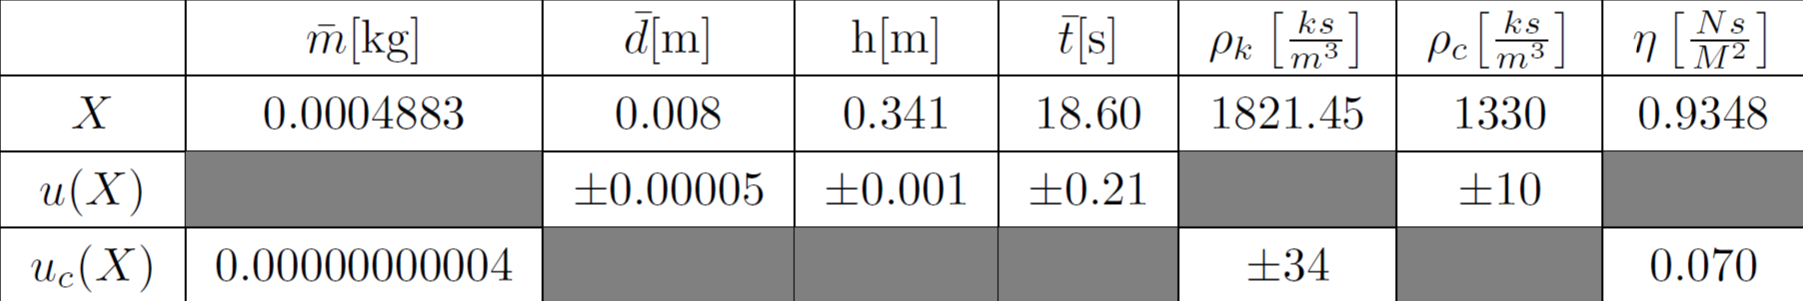
\includegraphics[scale=0.5]{t_b.png}
    \caption{asdasdadsasd}
% \end{figure}
% \begin{figure}
    \centering
    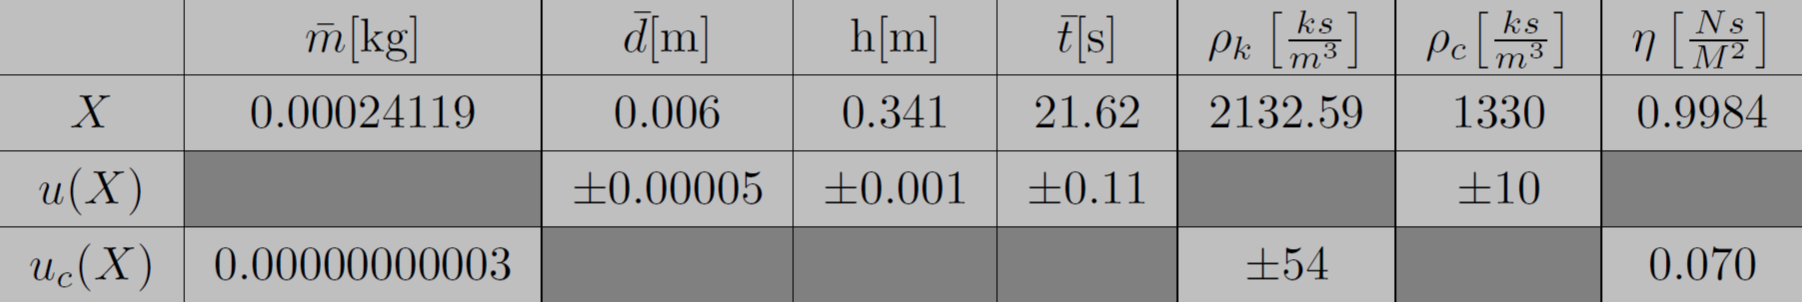
\includegraphics[scale=0.5]{t_c.png}
    \caption{asd}
% \end{figure}
% \vspace{-10ex}
% \begin{figure}
    \centering
    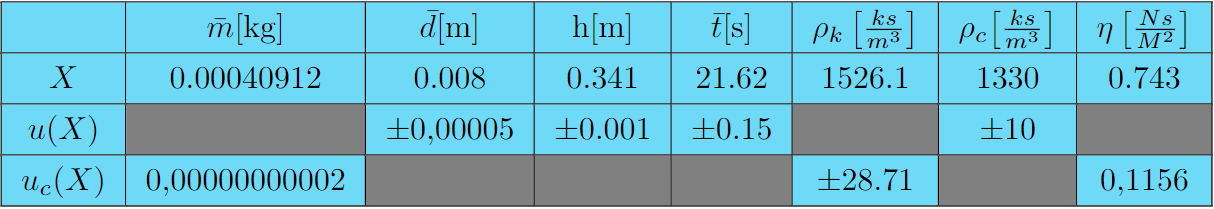
\includegraphics[scale=0.5]{t_n.png}
    \caption{aaaaa}
\end{figure}
%Uzylem screenow zakomentowanych tablic bo za chuja nie wiem jak je ustawic
% % POMIARY KULKI BIALEJ
% \begin{minipage}{0.48\textwidth}
%     % \rowcolors{2}{gray!5}{lightgray!30}
%     \begin{table}
%         \caption{Wyniki pomiaru kulki Białej}
%         \begin{tabular}{|l|r|r|r|}
%             \hline
%             Nr & d[m] & m[kg] & t[s] \\ \hline
%             1 & 0.008 & 0.000486  & 18.61 \\ \hline
%             2 & 0.008 & 0.00048   & 18.48 \\ \hline
%             3 & 0.008 & 0.0004824 & 20.36 \\ \hline
%             4 & 0.008 & 0.0004844 & 18.18 \\ \hline
%             5 & 0.008 & 0.000498  & 18.14 \\ \hline
%             6 & 0.008 & 0.0004916 & 18.38 \\ \hline
%             7 & 0.008 & 0.0004924 & 18.9  \\ \hline
%             8 & 0.008 & 0.0004954 & 18.16 \\ \hline
%             9 & 0.008 & 0.0004812 & 18.25 \\ \hline
%             10& 0.008 & 0.0004916 & 18.5  \\ \hline
%             Srednia: & 0.008 & 0.0004883 & 18.596 \\ \hline
%         \end{tabular}%
%         \label{tab:Tabela Pomiarow Kulki Bialej}%
%     \end{table}%
% \end{minipage}
% % POMIARY KULKI BIALEJ


% % POMIARY KULKI CZARNEJ
% \begin{minipage}{0.48\textwidth}
%     % \rowcolors{2}{gray!70}{lightgray!80}
%     \begin{table}
%         \caption{Wyniki pomiaru kulki Czarnej}
%         \begin{tabular}{|l|r|r|r|}
%             \hline
%             Nr& d[m] & m[kg] & t[s] \\ \hline
%             1 & 0.006 & 0.0002364 & 21.83 \\ \hline
%             2 & 0.006 & 0.000235  & 22.24 \\ \hline
%             3 & 0.006 & 0.0002516 & 21.61 \\ \hline
%             4 & 0.006 & 0.0002474 & 21.56 \\ \hline
%             5 & 0.006 & 0.0002464 & 21.67 \\ \hline
%             6 & 0.006 & 0.0002418 & 21.3  \\ \hline
%             7 & 0.006 & 0.0002376 & 21.57 \\ \hline
%             8 & 0.006 & 0.0002358 & 21.18 \\ \hline
%             9 & 0.006 & 0.0002422 & 22.08 \\ \hline
%             10& 0.006 & 0.0002377 & 21.16 \\ \hline
%             Srednia: & 0.006 & 0.00024119 & 21.62 \\ \hline
%         \end{tabular}%
%         \label{tab:Tabela Pomiarow Kulki Czarnej}%
%     \end{table}%
% \end{minipage}
% % POMIARY KULKI CZARNEJ

% % \vspace{-50ex}
% % POMIARY KULKI NIEBIESKIEJ
% % \begin{minipage}[0.33\textwidth]
% %     \rowcolors{2}{cyan!90}{cyan!40}
% %     \begin{table}[h]    
% %         \caption{Wyniki pomiaru kulki Niebieskiej}
% %         \begin{tabular}{|l|r|r|r|}
% %             \hline
% %             Nr pomiaru & d[m] & m[kg] & t[s] \\ \hline
% %             1 & 0.006 & 0.0002364 & 21.83 \\ \hline
% %             2 & 0.006 & 0.000235  & 22.24 \\ \hline
% %             3 & 0.006 & 0.0002516 & 21.61 \\ \hline
% %             4 & 0.006 & 0.0002474 & 21.56 \\ \hline
% %             5 & 0.006 & 0.0002464 & 21.67 \\ \hline
% %             6 & 0.006 & 0.0002418 & 21.3  \\ \hline
% %             7 & 0.006 & 0.0002376 & 21.57 \\ \hline
% %             8 & 0.006 & 0.0002358 & 21.18 \\ \hline
% %             9 & 0.006 & 0.0002422 & 22.08 \\ \hline
% %             10& 0.006 & 0.0002377 & 21.16 \\ \hline
% %             Srednia: & 0.006 & 0.00024119 & 21.62 \\ \hline
% %         \end{tabular}%
% %         \label{tab:Tabela Pomiarow Kulki Niebieskiej}%
% %     \end{table}%
% % \end{minipage}
% % POMIARY KULKI NIEBIESKIEJ

% \newpage

% OTRZYMANE POMIARY I ICH OPRACOWANIE
%------------------------------------------------------------------
\end{document}
